\section{WebService} % (fold)
\label{sec:webservice}

% section webservice (end)

As funcionalidades implementadas no \emph{BillMate}, podem ser acedidas por aplicações terceiras. Isto deve-se ao facto de se ter implementado um \emph{WebService}. Esta solução permite que tais aplicações possam comunicar com o \emph{BillMate} via \emph{HTTP} de forma normalizada e sem recurso a um \emph{browser}.

Para que se possa aceder a aplicação criada foi criada uma \emph{API REST}. Esta \emph{API} destaca-se pelos seguintes aspetos:

\begin{description}
  \item[Nomes em vez de Verbos] Ao usar nomes, tem-se URLs mais simples e mais intuitivos. Estes são escritos no formato \verb%/resource/:id/action% em que \verb%id% e \verb%action% são argumentos opcionais. Caso isto aconteça será retornado uma coleção do tipo do \emph{resource} especificado. Outros argumentos deverão ser passados por parâmetros

  \item[Métodos \emph{HTTP}] Ao simplificar o URL, passou a ser necessário arranjar mecanismos que traduzissem o mesmo URL numa ação de um controlador. A solução passa por usar os métodos \emph{HTTP} (GET, POST, PUT e DELETE). Ambos os verbos são baseados nas operações CRUD. A Tabela ~\ref{table:rest_methods}

  \item[Versões] A cada \emph{API} está associada uma versão, desta forma sempre que houver atualizações na aplicação, será mais fácil para outros programadores descobrirem a razão pela qual um operação antiga responde com mensagens de insucesso

  \item[Autenticação] Todos os pedidos feitos tem que ser acompanhados com um email e com um \emph{token}. Estes terão quase o mesmo efeito que uma sessão, permitindo que seja possível associar uma ação a um utilizador. Para se obter o \emph{token} é necessário efetuar \emph{Login} ou \emph{Register} a partir da \emph{API}
\end{description}


\begin{table}[ht]
	\label{table:rest_methods}
	\centering
	\begin{tabular}{ccccc}
		\hline
		\textbf{Resource} & \textbf{GET} & \textbf{POST} & \textbf{PUT} & \textbf{DELETE} \\
		\hline
		\textbf{/expense} & \specialcell{Lista todas\\as despesas} & Cria uma despesa & \specialcell{Atualiza todas\\ as despesas} &\specialcell{Apaga todas\\ as despesas}\\
		\hline
		\textbf{/expense/123} & \specialcell{Mostra a despesa\\ com o id 123} & & \specialcell{Atualiza a despesa\\ com o id 123} &\specialcell{Apaga a despesa\\ com o id 123}\\
		\hline
	\end{tabular}
\end{table}

Até ao momento a \emph{API} responde aos seguintes pedidos:

\begin{description}
	\item[POST] /api/v1/login
	\item[POST] /api/v1/register
	\item[GET POST] /api/v1/expense
	\item[GET] /api/v1/expense/:expense\_id
	\item[GET] /api/v1/circles/circle\_id
	\item[GET POST] /api/v1/house
	\item[GET] POST] /api/v1/collective
	\item[GET] /api/v1/circles/circle\_id/expense
\end{description}

\subsection{Mecanismo de Autenticação} % (fold)
\label{sub:mecanismo_de_autentica_o}

Na secção ~\ref{sec:webservice} é referido um método de autenticação através da \emph{API}, através do pedido \verb%POST /api/v1/login%. Contudo, para aplicações terceiras, esta solução acabar por não ser a melhor escolha no que diz respeito à autenticação, pois o utilizador acabar por não usufruir da aplicação, com receio de ver as suas credênciais de acesso guardadas e manipuladas por outras entidades alheias ao \emph{BillMate}.

A solução para o problema, resume-se em implementat um mecanismo de autenticação semelhante ao OAuth. Sempre que existe a necessidade de autenticar-se no \emph{BillMate} a partir de outras aplicações, o utilizador é reencaminhado para uma página de \emph{Login} gerida pelo \emph{BillMate}. No \emph{URL} de \emph{Login} deverá estar presente como parâmetro um \emph{URL de Callback}. Após autenticação, o utilizador é novamente reencaminhado para o endereço de \emph{Callback}, como parâmetros GET um  \emph{token} e o \emph{email} do utilizador. Todas as outras operações oferecidas pela \emph{API}, passam a estar disponiveis para essas aplicações.

Na figura ~\ref{fig:oauth} é representado o comportamento de um cliente \emph{OAuth} com o respetivo servidor.

\begin{figure}[ht]
	\centering
	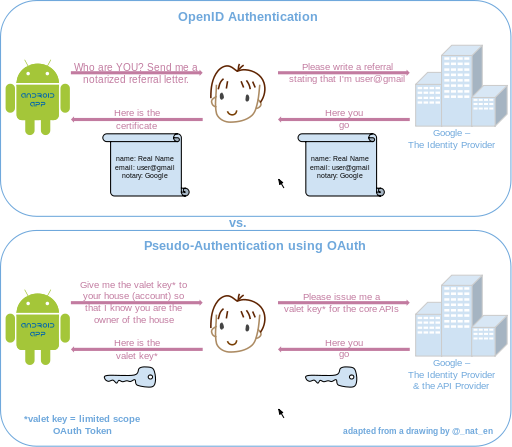
\includegraphics[width=.8\textwidth]{images/oauth}
	\caption{Funcionamento do \emph{OAuth}}
	\label{fig:oauth}
\end{figure}

% subsection mecanismo_de_autentica_o (end)
